% Figure from MATH 591 notes, section 8. Compile with the notes preamble.
\begin{tikzpicture}[scale=0.85]
\draw[gray!45] (-2.25,0) -- (2.25,0);
\draw[gray!70] (0,0) circle (1);
\draw[orange!80!black,thin] (0,1) -- (0,0) -- (0,-1);
\foreach \a/\u in {30/1.732, 150/-1.732, -30/0.577, 210/-0.577} {
  \draw[orange!80!black,thin] (0,1) -- (\u,0) -- (\a:1);
  \fill[violet!75!black] (\a:1) circle (1.2pt);
  \fill[teal!60!black] (\u,0) circle (1.2pt); }
\fill[violet!75!black] (0,-1) circle (1.4pt);
\fill[teal!60!black] (0,0) circle (1.4pt);
\draw[fill=white,thick] (0,1) circle (2.3pt);
\node[font=\footnotesize,anchor=south] at (0,1.13) {$N$ (omitted)};
\node[font=\footnotesize,anchor=north east] at (-0.06,-1.04) {$S$};
\node[font=\footnotesize,anchor=north west] at (0.07,-0.04) {$0$};
\node[font=\footnotesize,align=center,anchor=north] at (0,-1.75) {$\sigma_N(x,y)=\dfrac{x}{1-y}$\\[1pt] on $S^1\setminus\{N\}$\\[2pt] $S\mapsto0$; lower half $\to(-1,1)$};
\begin{scope}[shift={(6.4,0)}]
\draw[gray!45] (-2.25,0) -- (2.25,0);
\draw[gray!70] (0,0) circle (1);
\draw[teal!55!black,thin] (0,-1) -- (0,0) -- (0,1);
\foreach \a/\u in {30/0.577, 150/-0.577, -30/1.732, 210/-1.732} {
  \draw[teal!55!black,thin] (0,-1) -- (\u,0) -- (\a:1);
  \fill[violet!75!black] (\a:1) circle (1.2pt);
  \fill[teal!60!black] (\u,0) circle (1.2pt); }
\fill[violet!75!black] (0,1) circle (1.4pt);
\fill[teal!60!black] (0,0) circle (1.4pt);
\draw[fill=white,thick] (0,-1) circle (2.3pt);
\node[font=\footnotesize,anchor=north] at (0,-1.13) {$S$ (omitted)};
\node[font=\footnotesize,anchor=south east] at (-0.06,1.04) {$N$};
\node[font=\footnotesize,anchor=south west] at (0.07,0.05) {$0$};
\node[font=\footnotesize,align=center,anchor=north] at (0,-1.75) {$\sigma_S(x,y)=\dfrac{x}{1+y}$\\[1pt] on $S^1\setminus\{S\}$\\[2pt] $N\mapsto0$; upper half $\to(-1,1)$};
\end{scope}
\end{tikzpicture}
